% =====================================================================
%  PostLab 2 — Filtro activo paso bajo de segundo orden
%  Instrumentación Electrónica · Grado en Física · Universidad de Salamanca
%  Compilar con pdfLaTeX (dos pasadas):  latexmk -pdf main.tex
% =====================================================================
\documentclass[a4paper,11pt]{article}

% ---------- Idioma, codificación y tipografía ------------------------
\usepackage[T1]{fontenc}
\usepackage[utf8]{inputenc}
\usepackage[spanish,es-noshorthands,es-tabla,es-nodecimaldot]{babel}
\usepackage{amsmath}
\usepackage{newpxtext}
\usepackage{newpxmath}
\usepackage[protrusion=true,expansion=true]{microtype}
\linespread{1.06}

% ---------- Página ---------------------------------------------------
\usepackage[a4paper,left=2.6cm,right=2.6cm,top=2.7cm,bottom=2.6cm,headheight=14pt]{geometry}
\setlength{\parindent}{0pt}
\setlength{\parskip}{0.55em}

% ---------- Matemáticas y unidades -----------------------------------
\usepackage{siunitx}
\sisetup{
  output-decimal-marker = {,},
  group-minimum-digits  = 5,
  group-separator       = {\,},
  separate-uncertainty  = true,
  per-mode              = symbol,
  range-phrase          = {--},
  list-final-separator  = { y },
  exponent-product      = \cdot
}
\DeclareSIUnit\decada{\text{década}}
\DeclareSIUnit\dB{dB}

% ---------- Color ----------------------------------------------------
\usepackage[table]{xcolor}
\definecolor{navy}{HTML}{1B365D}     % tinta principal (títulos, datos)
\definecolor{azul}{HTML}{3E7CB1}     % acento (modelo teórico)
\definecolor{acero}{HTML}{7D9CC0}    % acento secundario
\definecolor{bruma}{HTML}{C9D6E6}    % filetes
\definecolor{fondo}{HTML}{EEF3F9}    % fondos de cajas
\definecolor{gris}{HTML}{8A939C}     % datos sin corregir, notas

% ---------- Figuras, tablas y gráficas -------------------------------
\usepackage{graphicx}
\usepackage{float}
\usepackage{booktabs}
\usepackage{array}
\usepackage{multirow}
\usepackage[font=small,labelfont={color=navy,sc},labelsep=period,
            justification=justified,singlelinecheck=true]{caption}
\usepackage{subcaption}
\captionsetup[sub]{font=footnotesize,labelfont={color=navy}}
\usepackage{tikz}
\usetikzlibrary{calc,positioning,babel}
\usepackage[american,siunitx]{circuitikz}
\usepackage{pgfplots}
\pgfplotsset{compat=1.18}
\usepgfplotslibrary{groupplots}
\usepackage[most]{tcolorbox}
\usepackage{enumitem}
\setlist{itemsep=0.25em,topsep=0.3em}

% ---------- Títulos de sección ---------------------------------------
\usepackage{titlesec}
\titleformat{\section}
  {\color{navy}\Large\bfseries}{\thesection.}{0.6em}{}
  [{\color{bruma}\titlerule[0.8pt]}]
\titlespacing*{\section}{0pt}{1.6em}{0.9em}
\titleformat{\subsection}
  {\color{navy}\large\bfseries}{\thesubsection.}{0.5em}{}
\titlespacing*{\subsection}{0pt}{1.2em}{0.4em}

% ---------- Encabezados ----------------------------------------------
\usepackage{fancyhdr}
\pagestyle{fancy}
\fancyhf{}
\renewcommand{\headrulewidth}{0.4pt}
\renewcommand{\headrule}{\hbox to\headwidth{\color{bruma}\leaders\hrule height \headrulewidth\hfill}}
\fancyhead[L]{\footnotesize\color{navy}\textsc{PostLab 2} \textperiodcentered{} Filtro activo paso bajo de segundo orden}
\fancyhead[R]{\footnotesize\color{gris}\textsc{Instrumentación Electrónica}}
\fancyfoot[C]{\footnotesize\color{navy}\thepage}

% ---------- Enlaces --------------------------------------------------
\usepackage[hidelinks]{hyperref}
\hypersetup{
  colorlinks=true, linkcolor=azul, urlcolor=azul, citecolor=azul,
  pdftitle={PostLab 2: filtro activo paso bajo de segundo orden},
  pdfauthor={Miguel Martín Cortés, Álvaro Montero Mateos, Daniel Martín Guerrero},
  pdfsubject={Instrumentación Electrónica, Universidad de Salamanca}
}

% ---------- Entornos propios -----------------------------------------
% Enunciado de cada pregunta del guion
\newtcolorbox{pregunta}{enhanced, breakable,
  colback=fondo, colframe=navy, boxrule=0pt, leftrule=2.4pt, arc=0pt,
  left=9pt, right=9pt, top=6pt, bottom=6pt, before skip=1.1em, after skip=0.8em,
  fontupper=\small\color{navy!85!black}}
% Resultado destacado
\newtcolorbox{resultado}{enhanced,
  colback=white, colframe=bruma, boxrule=0.6pt, arc=1.5pt,
  left=8pt, right=8pt, top=4pt, bottom=4pt, before skip=0.8em, after skip=0.8em,
  halign=center}

% ---------- Notación -------------------------------------------------
\newcommand{\Vin}{V_{\text{in}}}
\newcommand{\Vout}{V_{\text{out}}}
\newcommand{\pp}{\text{pp}}
\newcommand{\ef}{\text{ef}}
\newcommand{\dif}{\mathop{}\!\mathrm{d}}
\newcommand{\uA}{\textmu A741}

\begin{document}

% =====================================================================
%  PORTADA
% =====================================================================
\newgeometry{left=2.6cm,right=2.6cm,top=1.9cm,bottom=1.7cm}
\begin{titlepage}
\thispagestyle{empty}\setlength{\parskip}{0pt}%
\begin{tikzpicture}[remember picture,overlay]
  \fill[navy] ($(current page.north east)+(-1.25cm,-2.3cm)$) rectangle ($(current page.south east)+(-1.05cm,2.3cm)$);
  \fill[acero] ($(current page.north east)+(-0.85cm,-2.3cm)$) rectangle ($(current page.north east)+(-0.80cm,-9.0cm)$);
\end{tikzpicture}

\begin{minipage}[c]{0.5\textwidth}
  
\includegraphics[height=1.55cm]{figuras/logo_usal.png}
\end{minipage}\hfill
\begin{minipage}[c]{0.4\textwidth}\raggedleft
  
\includegraphics[height=1.15cm]{figuras/logo_ciencias.png}
\end{minipage}

\vspace{0.35cm}
{\color{bruma}\rule{\textwidth}{0.6pt}}

\vspace{0.25cm}
\begin{center}
  {\color{navy}\large\textsc{Universidad de Salamanca}}\\[0.2em]
  {\color{gris}\small\textsc{Facultad de Ciencias \textperiodcentered{} Grado en Física \textperiodcentered{} Segundo curso}}
\end{center}

\vspace{0.6cm}
\begin{center}
  {\color{azul}\large\textsc{Instrumentación Electrónica}}\\[0.25em]
  {\color{gris}\textsc{Laboratorio de circuitos, sesión 2}}

  \vspace{0.75cm}
  {\color{navy}\fontsize{27}{33}\selectfont\bfseries PostLab: filtro activo paso bajo\\[0.15em] de segundo orden\par}

  \vspace{0.55cm}
  {\color{acero}\rule{2.6cm}{1.2pt}}

  \vspace{0.45cm}
  {\itshape\color{navy!80!black}Medida de la respuesta en frecuencia, diagrama de Bode experimental\\
  y comparación con el modelo teórico del PreLab\par}

  \vspace{0.55cm}
  {\color{navy!85!black}\small
  $\displaystyle T(s)=\frac{T_0}{s^2+\dfrac{\omega_0}{Q}\,s+\omega_0^2}$\qquad\quad
  $\displaystyle \omega_0=\frac{1}{\sqrt{R_1R_2C_1C_2}}$\qquad\quad
  $\displaystyle K=1+\frac{R_A}{R_B}$\par}
\end{center}

\vspace{0.5cm}
\begin{tcolorbox}[enhanced, colback=fondo, colframe=fondo, arc=0pt, boxrule=0pt,
  borderline west={2.4pt}{0pt}{navy}, left=10pt, right=10pt, top=7pt, bottom=7pt]
  {\color{navy}\small\textsc{Resumen}}\par\vspace{0.2em}
  \footnotesize
  Se ha montado un filtro activo paso bajo de segundo orden con el amplificador operacional \uA{} y se ha medido el módulo de su función de transferencia entre \qty{20}{Hz} y \qty{10}{kHz}. La ganancia en banda pasante, \qty{7,89}{dB}, difiere en menos de \qty{0,1}{dB} de la prevista con los componentes medidos; el máximo, de \qty{14,43}{dB}, aparece en torno a \qty{774}{Hz} (teórico: \qty{13,97}{dB} a \qty{746}{Hz}); la frecuencia de corte se estima en \qty{1150}{Hz} (teórica: \qty{1187}{Hz}), y la banda atenuada cae con una pendiente de $\qty{-41,1(20)}{dB/\decada}$, compatible con los $\qty{-40}{dB/\decada}$ propios de un sistema de segundo orden. Se discute, además, por qué conviene medir valores eficaces cuando la señal es débil y cómo la mezcla de medidas pico a pico y eficaces introduce un error sistemático de $\qty{-9,03}{dB}$.
\end{tcolorbox}

\vfill
{\color{bruma}\rule{\textwidth}{0.6pt}}
\vspace{0.15cm}

\begin{minipage}[t]{0.40\textwidth}
  {\color{azul}\footnotesize\textsc{Autores}}\\[0.35em]
  \small
  Miguel Martín Cortés {\color{gris}\footnotesize(70974284X)}\\
  Álvaro Montero Mateos {\color{gris}\footnotesize(71096223A)}\\
  Daniel Martín Guerrero {\color{gris}\footnotesize(71063727Y)}\\[0.3em]
  {\color{gris}\footnotesize Grupo de laboratorio C.2}
\end{minipage}\hfill
\begin{minipage}[t]{0.50\textwidth}
  {\color{azul}\footnotesize\textsc{Profesores}}\\[0.35em]
  \small
  Yahya Moubarak Meziani\\
  María Susana Pérez Santos\\
  Jesús Enrique Velázquez Pérez\\[0.3em]
  {\color{gris}\footnotesize Departamento de Física Aplicada \textperiodcentered{} Área de Electrónica}
\end{minipage}

\vspace{0.4cm}
\begin{center}
  {\color{navy}\textsc{Informe de laboratorio (PostLab)}}\\[0.2em]
  {\color{gris}\small\textsc{Salamanca, curso 2026/2027}}
\end{center}
\end{titlepage}
\restoregeometry

\setcounter{page}{1}

% =====================================================================
\section{Introducción y descripción teórica}
% =====================================================================
Los objetivos de esta práctica son diseñar y montar un filtro pasa-baja de segundo orden. Además, se medirá su función de transferencia para distintas frecuencias.

Para ello se usará un osciloscopio, un generador de funciones, un multímetro, un entrenador, componentes pasivos y el amplificador operacional \uA.

A continuación se muestra el esquema del circuito montado en el laboratorio:

\begin{figure}[H]
\centering
\begin{circuitikz}[scale=0.92, transform shape, color=navy, line width=0.6pt]
  \ctikzset{bipoles/length=1.15cm, monopoles/ground/width=0.8}
  % Amplificador operacional (entrada no inversora arriba)
  \node[op amp, noinv input up, fill=fondo, scale=1.15] (OA) at (0,0) {\scriptsize\uA};
  % Entrada no inversora: red R1-R2-C2
  \draw (OA.+) -- ++(-2.1,0) coordinate (Vp);
  \draw (Vp) to[R, l_=$R_2$, *-] ++(-2.6,0) coordinate (Vx)
             to[R, l_=$R_1$, *-] ++(-2.6,0) coordinate (In);
  \draw (Vp) to[C, l_=$C_2$] ($(Vp)+(0,-3.4)$) coordinate (G1) node[ground]{};
  % Fuente de entrada
  \draw (In) to[sV, l_=$v_{\text{in}}$] (In |- G1) node[ground]{};
  % Salida y realimentación
  \draw (OA.out) -- ++(1.4,0) coordinate (Out) to[short, -o] ++(0.9,0) node[right]{$\Vout$};
  \draw (Out) node[circ]{};
  \draw (Vx) -- ++(0,2.2) coordinate (C1a) to[C, l=$C_1$] (C1a -| Out) -- (Out);
  \draw (OA.-) -- ++(-0.7,0) coordinate (Vm) -- ++(0,-1.25) coordinate (Vm2);
  \draw (Vm2) to[R, l_=$R_A$, *-] (Vm2 -| Out) -- (Out);
  \draw (Vm2) to[R, l=$R_B$] (Vm2 |- G1) node[ground]{};
  % Alimentación
  \draw (OA.up) -- ++(0,0.45) node[above]{\scriptsize $+V_{CC}$};
  \draw (OA.down) -- ++(0,-0.45) node[below]{\scriptsize $-V_{CC}$};
  % Nudos y patillas
  \node[above, font=\footnotesize] at ($(Vx)+(-0.35,0)$) {$V_x$};
  \node[above, font=\footnotesize] at ($(Vp)+(0.45,0)$) {$V_+$};
  \node[below left, font=\footnotesize] at ($(Vm)+(0,-0.05)$) {$V_-$};
  \node[font=\tiny, color=gris] at ($(OA.+)+(-0.3,0.17)$) {3};
  \node[font=\tiny, color=gris] at ($(OA.-)+(-0.3,0.17)$) {2};
  \node[font=\tiny, color=gris] at ($(OA.out)+(0.3,0.17)$) {6};
  \node[font=\tiny, color=gris] at ($(OA.up)+(0.2,0.3)$) {7};
  \node[font=\tiny, color=gris] at ($(OA.down)+(0.2,-0.3)$) {4};
\end{circuitikz}
\caption{Filtro pasa-baja de segundo orden montado en el laboratorio. Se indican los nudos empleados en el análisis del PreLab y las patillas del \uA{} utilizadas.}
\label{fig:circuito}
\end{figure}

La función de transferencia depende de los componentes del circuito $R_1,R_2,C_1,C_2,R_A,R_B$ y viene dada por la siguiente expresión:
\begin{equation}
    T(s) = \frac{\Vout}{\Vin}=\frac{T_0}{\omega_0^2+\dfrac{\omega_0 s}{Q}+s^2},
    \label{eq:T}
\end{equation}
donde, según se obtuvo en el PreLab,
\begin{equation}
    \omega_0=\frac{1}{\sqrt{R_1R_2C_1C_2}},\qquad
    T_0=K\omega_0^2,\qquad
    Q=\frac{\sqrt{R_1R_2C_1C_2}}{(R_1+R_2)C_2-\dfrac{R_A}{R_B}R_1C_1}.
    \label{eq:param}
\end{equation}
con $K=1+R_A/R_B$. El estudio teórico de la función de transferencia se realizó en el PreLab.

% =====================================================================
\section{Montaje y procedimiento de medida}
% =====================================================================
A continuación se dan los valores de los componentes usados en el circuito, medidos con el multímetro, junto con los valores nominales de la tabla~I del guion:

\begin{table}[H]
\centering
\renewcommand{\arraystretch}{1.25}
\begin{tabular}{@{}l *{6}{c}@{}}
  \toprule
  & $R_1$ [\unit{k\ohm}] & $R_2$ [\unit{k\ohm}] & $C_1$ [\unit{nF}] & $C_2$ [\unit{nF}] & $R_A$ [\unit{k\ohm}] & $R_B$ [\unit{k\ohm}] \\
  \midrule
  Nominal (tabla~I del guion) & \num{22} & \num{22} & \num{10} & \num{10} & \num{15} & \num{10} \\
  \rowcolor{fondo}
  Medido & \num{21.7} & \num{21.7} & \num{9.07} & \num{9.21} & \num{14.95} & \num{9.92} \\
  \bottomrule
\end{tabular}
\caption{Valores de los componentes usados en el circuito.}
\label{tab:datoscomp}
\end{table}

\begin{figure}[H]
  \centering
  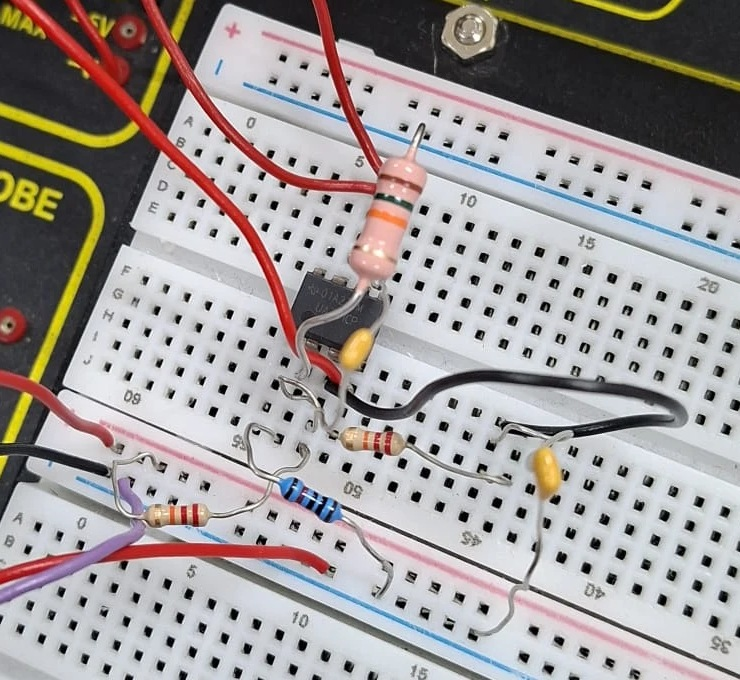
\includegraphics[width=0.44\textwidth]{figuras/montaje.jpg}
  \caption{Montaje del filtro en la placa de prototipos del entrenador A-TEK AT-700: el \uA{} en encapsulado DIP-8 y, a su alrededor, la red $R_1C_1$–$R_2C_2$ y el divisor $R_A$–$R_B$.}
  \label{fig:montaje}
\end{figure}

\subsection{Elección de \texorpdfstring{$R_A$}{RA} y \texorpdfstring{$R_B$}{RB}}

\begin{pregunta}
¿Puede el valor de $R_A$ acercarse al doble del de $R_B$? ¿Por qué? La razón debe buscarse de manera teórica usando los resultados obtenidos en el PreLab.
\end{pregunta}

No, y para verlo basta con que nos fijemos en los polos de $T(s)$, es decir, en las raíces de su denominador:
\begin{equation}
\begin{gathered}
  D(s)=s^2+\frac{\omega_0}{Q}\,s+\omega_0^2=0
  \quad\Longrightarrow\quad
  s_{1,2}=\sigma\pm j\omega_d ,\\
  \sigma=-\frac{\omega_0}{2Q},\qquad
  \omega_d=\omega_0\sqrt{1-\frac{1}{4Q^2}},
\end{gathered}
  \label{eq:polos}
\end{equation}
expresión válida para $|Q|>1/2$ (respuesta subamortiguada). Como cada polo aporta a la respuesta libre un término $e^{st}=e^{\sigma t}e^{j\omega_d t}$, una oscilación con envolvente $e^{\sigma t}$, todo depende del signo de $\sigma$, que es el contrario al de $Q$. Recordando lo que obtuvimos en el PreLab,
\begin{equation}
\begin{aligned}
  \frac{1}{Q}&=\frac{(R_1+R_2)\,C_2-\dfrac{R_A}{R_B}\,R_1C_1}{\sqrt{R_1R_2C_1C_2}}\\[4pt]
  &=2-\frac{R_A}{R_B}\qquad\text{(si $R_1=R_2$ y $C_1=C_2$)},
\end{aligned}
  \label{eq:Qsimple}
\end{equation}
lo que nos dice que el amortiguamiento es la diferencia entre la disipación en las resistencias y la realimentación positiva a través de $C_1$, que crece con $R_A/R_B$. Con componentes iguales dos a dos, como en la tabla~I, distinguimos tres regímenes (figura~\ref{fig:polos}):
\begin{itemize}
  \item $R_A<2R_B$: $Q>0$ y $\sigma<0$; los polos están en el semiplano izquierdo, la envolvente decae y el circuito filtra.
  \item $R_A=2R_B$: $1/Q=0$ y los polos caen en $\pm j\omega_0$; el pico $|T(j\omega_0)|=KQ$ diverge y el circuito oscila a $f_0$.
  \item $R_A>2R_B$: $Q<0$ y $\sigma>0$; los polos pasan al semiplano derecho y cualquier perturbación (ruido, el transitorio de encendido) crece exponencialmente hasta que la salida alcanza $\pm V_{CC}$ y el AO se satura.
\end{itemize}
En general, para que el filtro sea estable necesitamos
\begin{equation}
  \frac{R_A}{R_B}<\frac{(R_1+R_2)\,C_2}{R_1C_1},
\end{equation}
que con los componentes medidos fija el límite en $R_A/R_B<\num{2.031}$. Nuestro cociente, $R_A/R_B=\num{1.507}$, queda holgadamente por debajo y da $Q=\num{1.92}$: polos complejos conjugados en el semiplano izquierdo, con $\sigma=-\qty{1310}{s^{-1}}$, de modo que cualquier transitorio se extingue en unos $1/|\sigma|\approx\qty{0.76}{ms}$.

\begin{figure}[htbp]
\centering
\pgfplotsset{
  colormap={fase}{rgb=(0.970,0.213,0.213) rgb=(0.970,0.970,0.213) rgb=(0.213,0.970,0.213)
                  rgb=(0.213,0.970,0.970) rgb=(0.213,0.213,0.970) rgb=(0.970,0.213,0.970)
                  rgb=(0.970,0.213,0.213)}}
\begin{tikzpicture}
\begin{groupplot}[
  group style={group size=3 by 1, horizontal sep=0.45cm, y descriptions at=edge left},
  width=5.35cm, height=5.35cm,
  xmin=-1.6, xmax=1.6, ymin=-1.6, ymax=1.6, axis equal image,
  xtick={-1,0,1}, ytick={-1,0,1},
  tick label style={font=\footnotesize, color=navy!80!black},
  label style={font=\small, color=navy},
  title style={font=\small, color=navy, yshift=-2pt},
  xlabel={$\operatorname{Re}s/\omega_0$}, ylabel={$\operatorname{Im}s/\omega_0$},
  axis line style={gris!70}, tick style={gris!70}, enlargelimits=false,
  axis on top,
  /pgf/number format/use comma,
]
\newcommand{\marcas}[2]{%
  \addplot[white, line width=0.5pt, opacity=0.85] coordinates {(0,-1.6) (0,1.6)};
  \addplot[white, densely dashed, line width=0.6pt, domain=0:360, samples=120] ({cos(x)},{sin(x)});
  \addplot[only marks, mark=x, mark size=3.6pt, navy, line width=2.6pt] coordinates {(#1,#2) (#1,-#2)};
  \addplot[only marks, mark=x, mark size=3.2pt, white, line width=1.3pt] coordinates {(#1,#2) (#1,-#2)};
}
\nextgroupplot[title={(a) $Q=\num{1.92}$}]
  \addplot graphics[xmin=-1.6, xmax=1.6, ymin=-1.6, ymax=1.6] {figuras/fase_estable.png};
  \marcas{-0.2599}{0.9656}
\nextgroupplot[title={(b) $Q\to\infty$}]
  \addplot graphics[xmin=-1.6, xmax=1.6, ymin=-1.6, ymax=1.6] {figuras/fase_limite.png};
  \marcas{0}{1}
\nextgroupplot[title={(c) $Q=\num{-2.15}$},
  colorbar, colormap name=fase, point meta min=-3.14159, point meta max=3.14159,
  colorbar style={width=0.22cm, ytick={-3.14159,0,3.14159}, yticklabels={$-\pi$,$0$,$\pi$},
    ylabel={$\arg T(s)$}, ylabel style={font=\small, color=navy},
    tick label style={font=\footnotesize, color=navy!80!black}, axis line style={gris!70}}]
  \addplot graphics[xmin=-1.6, xmax=1.6, ymin=-1.6, ymax=1.6] {figuras/fase_inestable.png};
  \marcas{0.2328}{0.9725}
\end{groupplot}
\end{tikzpicture}
\caption{Retratos de fase de $T(s)$ con los componentes medidos: cada punto $s$ se colorea según $\arg T(s)$, y alrededor de cada polo ($\times$) el círculo cromático se recorre una vez. Los polos se mueven sobre la circunferencia $|s|=\omega_0$ (discontinua) al variar $R_A/R_B$: (a) nuestro montaje, $R_A/R_B=\num{1.507}$, estable; (b) límite de estabilidad, $R_A/R_B=\num{2.031}$, oscilador; (c) $R_A/R_B=\num{2.5}$, inestable: la salida crece hasta saturar el AO.}
\label{fig:polos}
\end{figure}

Incluso sin llegar al límite, en la práctica no nos conviene acercarnos a él, porque el filtro se vuelve muy sensible a las tolerancias. Si derivamos $Q=1/(2-R_A/R_B)$, obtenemos $\dif Q/Q=Q\,\dif(R_A/R_B)$, de modo que con $R_A/R_B=\num{1.5}$ ($Q=2$) un error del \qty{1}{\percent} en $R_A$ altera $Q$ un \qty{3}{\percent}, pero con $R_A/R_B=\num{1.9}$ ($Q=10$, pico de \qty{20}{dB} sobre la banda pasante) ese mismo \qty{1}{\percent} lo altera un \qty{19}{\percent}, y la tolerancia habitual de las resistencias (\qty{5}{\percent}) bastaría para volver inestable el circuito.

\subsection{Procedimiento y decisiones tomadas durante la medida}

Se aplicó a la entrada una señal sinusoidal del generador, que se midió siempre en el canal~1 del osciloscopio, y la salida del filtro en el canal~2. En la banda pasante y en torno a la resonancia se trabajó con $\Vin=\qty{1.04}{V_{pp}}$, y se comprobó en cada punto que la salida no se recortaba (la mayor amplitud, $\qty{5.48}{V_{pp}}$ a \qty{774}{Hz}, queda muy lejos de la saturación del AO). El rango cubierto fue \qtyrange{20}{10000}{Hz}; la figura~\ref{fig:osc}\,(a) muestra, como comprobación adicional, que a \qty{12.9}{Hz} la ganancia sigue siendo la de la banda pasante.

A partir de \qty{2780}{Hz}, con la salida ya atenuada hasta las décimas de voltio, la forma de onda dejó de verse limpia: el ruido la deformaba y la lectura pico a pico se volvía inestable (figura~\ref{fig:osc}\,(d)). Sobre la marcha, hicimos dos cambios:
\begin{enumerate}[label=(\roman*)]
  \item \textbf{Aumentamos la amplitud de entrada} hasta $\Vin=\qty{2.02}{V_{pp}}$. Como el filtro es lineal, $|T|$ no depende de la amplitud, y así la señal útil de salida gana terreno frente a un ruido que no cambia.
  \item \textbf{Pasamos a medir el valor eficaz de la salida}, que es mucho menos sensible al ruido que el pico a pico, como se discute en la primera pregunta del bloque~1.
\end{enumerate}
La entrada, en cambio, la seguimos anotando como valor pico a pico, así que en esos puntos el cociente mezcla dos tipos de medida. Lo corregimos en la sección~\ref{sec:bloque1}.

\begin{figure}[tbp]
  \centering
  \begin{subfigure}[t]{0.485\textwidth}
    \centering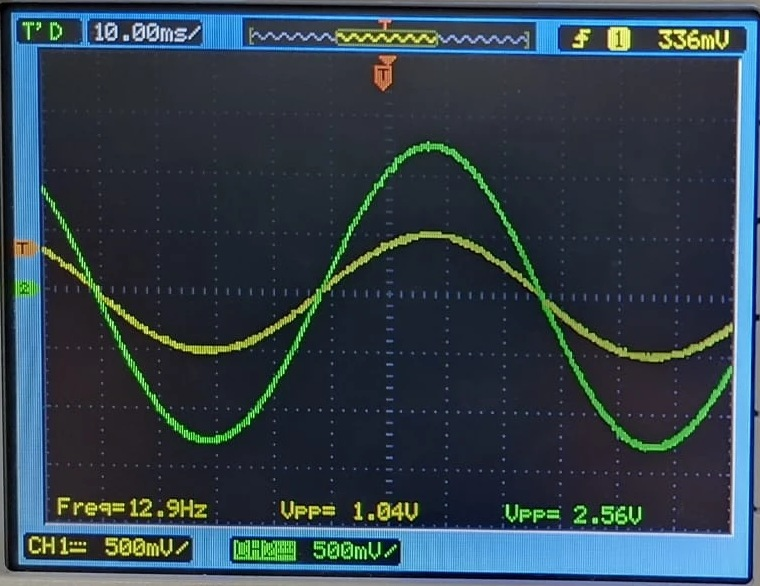
\includegraphics[width=\linewidth]{figuras/osc_12Hz.jpg}
    \caption{\qty{12.9}{Hz}: banda pasante; $\Vout/\Vin=\num{2.56}/\num{1.04}$, \qty{7.82}{dB}.}
  \end{subfigure}\hfill
  \begin{subfigure}[t]{0.485\textwidth}
    \centering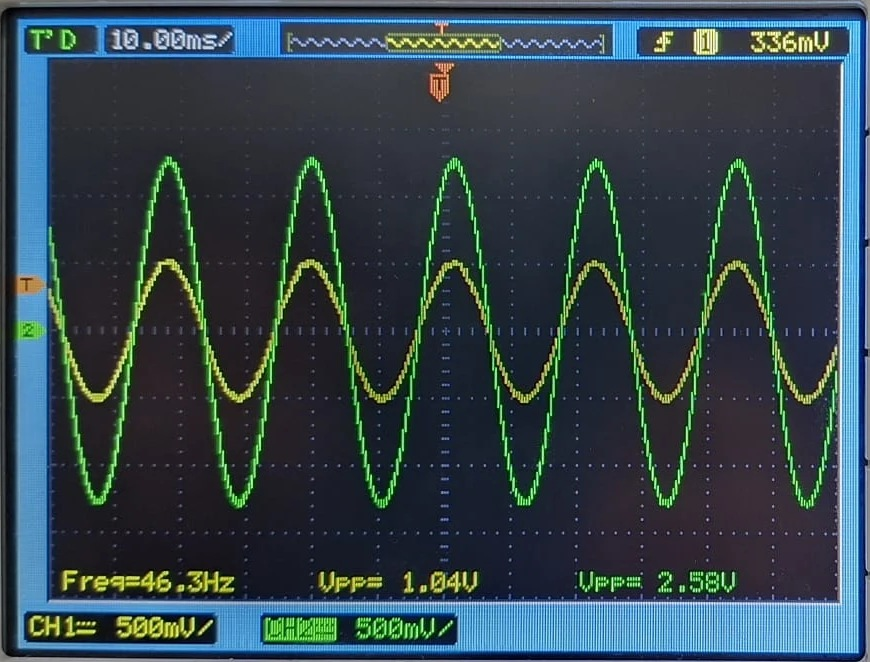
\includegraphics[width=\linewidth]{figuras/osc_46Hz.jpg}
    \caption{\qty{46.3}{Hz}: banda pasante; $\Vout/\Vin=\num{2.58}/\num{1.04}$, \qty{7.89}{dB}, en fase.}
  \end{subfigure}\\[0.7em]
  \begin{subfigure}[t]{0.485\textwidth}
    \centering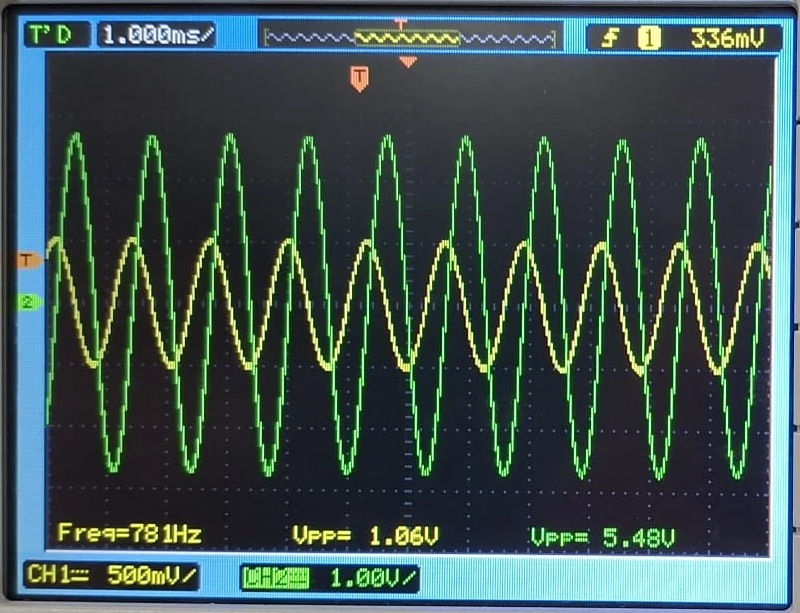
\includegraphics[width=\linewidth]{figuras/osc_781Hz.jpg}
    \caption{\qty{781}{Hz}: cerca del máximo; $\Vout=\qty{5.48}{V_{pp}}$ (escala de \qty{1}{V/div}) y desfase próximo a \ang{90}.}
  \end{subfigure}\hfill
  \begin{subfigure}[t]{0.485\textwidth}
    \centering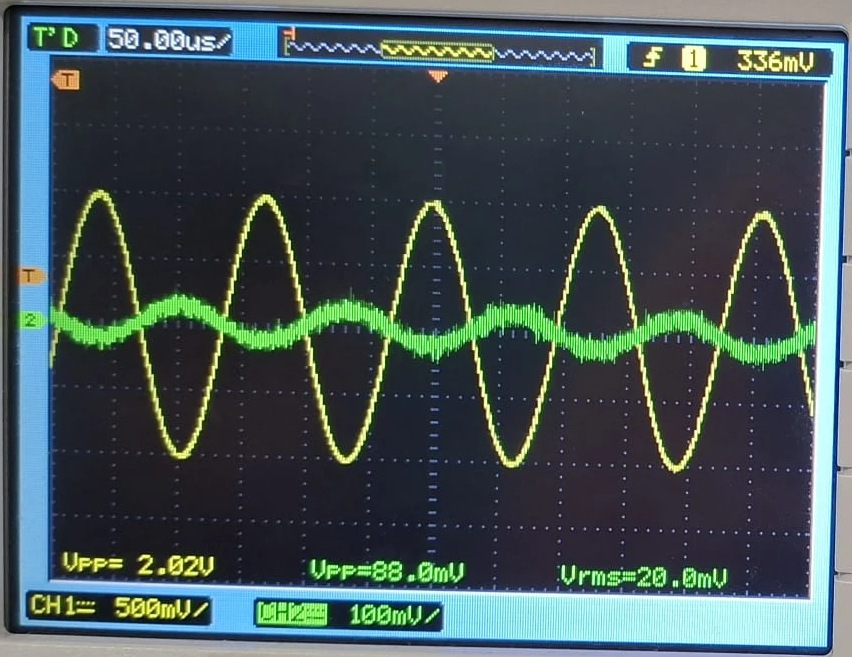
\includegraphics[width=\linewidth]{figuras/osc_7740Hz.jpg}
    \caption{$\approx\qty{7.7}{kHz}$ (\qty{50}{\micro s/div}): banda atenuada; salida ruidosa, en oposición de fase, con \qty{88.0}{mV_{pp}} pero solo \qty{20.0}{mV_{ef}}.}
  \end{subfigure}
  \caption{Capturas del osciloscopio (canal~1, amarillo: entrada; canal~2, verde: salida) en las tres regiones del diagrama de Bode. El disparo se realiza en todas ellas sobre el canal~1, con un nivel de \qty{336}{mV}.}
  \label{fig:osc}
\end{figure}

\clearpage
% =====================================================================
\section{Preguntas bloque 1}
\label{sec:bloque1}
% =====================================================================

\begin{pregunta}
¿Puede ser conveniente medir valores eficaces (\emph{root mean square}) de las tensiones de entrada/salida en vez de medidas pico a pico? ¿Por qué y en qué circunstancias?
\end{pregunta}

Sí, y en nuestro montaje resultó imprescindible a alta frecuencia. Para una sinusoide limpia, $V_{\pp}=2\sqrt{2}\,V_{\ef}$ y ambas medidas son equivalentes; pero si a la señal se le superpone ruido, el máximo y el mínimo los marcan sus picos, y $V_{\pp}$ queda sesgada al alza y fluctúa. El valor eficaz, en cambio, promedia todas las muestras y, si el ruido es incorrelado con la señal, ambos se suman en cuadratura:
\begin{equation}
  V_{\ef}^2=V_{s,\ef}^2+V_{n,\ef}^2 ,
  \label{eq:cuadratura}
\end{equation}
de modo que un ruido de la cuarta parte de la señal apenas aumenta $V_{\ef}$ un \qty{3}{\percent}. Lo vemos en la figura~\ref{fig:osc}\,(d): a $f\approx\qty{7.74}{kHz}$ la salida marca \qty{88.0}{mV_{pp}} pero solo \qty{20.0}{mV_{ef}}, cuando una sinusoide pura tendría \qty{56.6}{mV_{pp}}; el modelo predice \qty{19.4}{mV_{ef}}, así que el valor eficaz acierta con un \qty{3}{\percent} de error, mientras que el pico a pico daría unos \qty{4}{dB} de más.

Por tanto, nos conviene medir valores eficaces cuando la señal es pequeña y comparable al ruido, como en la banda atenuada (aquí, por encima de unos \qty{2}{kHz}), con acoplamiento en alterna y midiendo ambos canales del mismo modo. En la banda pasante, la medida pico a pico es igual de válida y más inmediata.

\begin{pregunta}
Con un valor alto de las señales de entrada y salida, ¿cambia el valor de la ganancia en dB usando medidas de valores eficaces frente al resultado obtenido usando medidas pico a pico? Justifíquese.
\end{pregunta}

No, siempre que las dos señales sean sinusoidales y se midan del mismo modo. Como el filtro es lineal e invariante, la salida es una sinusoide de la misma frecuencia que la entrada y, para ambas, $V_{\pp}=2\sqrt2\,V_{\ef}$, de modo que el factor se cancela en el cociente:
\begin{equation}
  |T|_{\text{dB}}
  =20\log_{10}\frac{V_{\text{out},\pp}}{V_{\text{in},\pp}}
  =20\log_{10}\frac{2\sqrt2\,V_{\text{out},\ef}}{2\sqrt2\,V_{\text{in},\ef}}
  =20\log_{10}\frac{V_{\text{out},\ef}}{V_{\text{in},\ef}} .
\end{equation}
Con señales altas el ruido es despreciable: por \eqref{eq:cuadratura}, solo altera el valor eficaz en $10\log_{10}(1+\rho^2)\approx\qty{4.3}{dB}\cdot\rho^2$, con $\rho=V_{n,\ef}/V_{s,\ef}$, menos de \qty{0.001}{dB} para $\rho=\qty{1}{\percent}$. Las medidas solo discreparían si la onda dejara de ser sinusoidal, por ejemplo por recorte en la alimentación (que se vigiló en todo momento) o por el \emph{slew rate} del \uA{}, que no limita aquí: el caso más exigente, $\qty{5.48}{V_{pp}}$ a \qty{774}{Hz}, requiere $2\pi fA\approx\qty{0.013}{V/\micro s}$, frente a unos \qty{0.5}{V/\micro s}.

Lo que no puede hacerse es mezclar ambos tipos de medida, ya que
\begin{equation}
  20\log_{10}\frac{V_{\text{out},\ef}}{V_{\text{in},\pp}}
  =|T|_{\text{dB}}-20\log_{10}\!\left(2\sqrt2\right)
  =|T|_{\text{dB}}-\qty{9.03}{dB}.
\end{equation}
Es lo que ocurría en nuestros registros a partir de \qty{2780}{Hz}, donde $\Vin$ se anotó pico a pico y $\Vout$ como valor eficaz. Lo corregimos convirtiendo la entrada, $V_{\text{in},\ef}=\qty{2.02}{V}/(2\sqrt2)=\qty{0.714}{V}$: a \qty{7740}{Hz}, por ejemplo, se pasa de $\qty{-40.09}{dB}$ a $\qty{-31.06}{dB}$, frente a $\qty{-31.31}{dB}$ del modelo. Todas las tablas y gráficas que siguen usan los valores corregidos.

\begin{pregunta}
Empíricamente se encuentra que, bajo ciertas condiciones, la medida de frecuencia que realiza el osciloscopio puede ser menos estable si se usa uno de los dos canales (es decir, realizar el \emph{triggering} es más difícil). ¿Qué canal debe ser usado para medir la frecuencia: aquel en el que se mide la tensión de entrada o aquel en el que se mide la de salida del filtro? Justifíquese.
\end{pregunta}

Debe usarse el canal de la tensión de entrada (el canal~1, como además exige el guion). Un sistema lineal e invariante no crea frecuencias nuevas, así que ambas señales tienen la misma frecuencia; la diferencia está en la calidad de la señal sobre la que trabajan el disparo y el frecuencímetro, que detectan sus cruces por el nivel de disparo:
\begin{itemize}
  \item La entrada procede directamente del generador, es prácticamente limpia y su amplitud es constante en todo el barrido, de modo que un único nivel de disparo (\qty{336}{mV} en todas las capturas) sirve para cualquier frecuencia.
  \item La salida varía en más de \qty{45}{dB} a lo largo del barrido y, en la banda atenuada, se reduce a unas decenas de milivoltios con un ruido de unos pocos milivoltios, comparable a la histéresis del comparador. Cerca de cada cruce, el ruido hace que la señal atraviese el nivel varias veces: hay disparos falsos, la traza «baila» y la frecuencia medida fluctúa; además, habría que reajustar el nivel en cada punto.
\end{itemize}
La figura~\ref{fig:osc}\,(d) lo ilustra: pese a lo ruidosa que es la salida, la imagen es estable porque el disparo se realiza sobre la entrada.

\subsection{Tablas de medidas}

\begin{pregunta}
Dense las citadas tablas con los valores de las medidas.
\end{pregunta}

Las tablas~\ref{tab:bajas} y~\ref{tab:decadas} recogen las medidas tal y como se tomaron en el laboratorio. Junto a cada punto se da el módulo experimental, $|T|=20\log_{10}(\Vout/\Vin)$, y el previsto por \eqref{eq:T} con los componentes medidos ($K=\num{2.507}$, $f_0=\qty{802.5}{Hz}$, $Q=\num{1.924}$).

\begin{table}[H]
\centering
\small
\renewcommand{\arraystretch}{1.12}
\setlength{\tabcolsep}{5pt}
\begin{tabular}{@{}*{3}{S[table-format=3.1] S[table-format=1.2] S[table-format=1.2]}@{}}
  \toprule
  \multicolumn{3}{c}{Barrido A} & \multicolumn{3}{c}{Barrido B} & \multicolumn{3}{c}{Barrido C}\\
  \cmidrule(lr){1-3}\cmidrule(lr){4-6}\cmidrule(lr){7-9}
  {$f$ [\unit{Hz}]} & {$\Vout$ [\unit{V}]} & {$|T|$ [\unit{dB}]} &
  {$f$ [\unit{Hz}]} & {$\Vout$ [\unit{V}]} & {$|T|$ [\unit{dB}]} &
  {$f$ [\unit{Hz}]} & {$\Vout$ [\unit{V}]} & {$|T|$ [\unit{dB}]} \\
  \midrule
  20 & 2.58 & 7.89 & 30 & 2.58 & 7.89 & 40 & 2.58 & 7.89 \\
  \rowcolor{fondo}
  22.9 & 2.58 & 7.89 & 32.9 & 2.58 & 7.89 & 42.9 & 2.58 & 7.89 \\
  26.7 & 2.58 & 7.89 & 36.7 & 2.58 & 7.89 & 46.7 & 2.58 & 7.89 \\
  \rowcolor{fondo}
  31.5 & 2.58 & 7.89 & 41.5 & 2.57 & 7.86 & 51.5 & 2.58 & 7.89 \\
  37.8 & 2.58 & 7.89 & 47.8 & 2.58 & 7.89 & 57.8 & 2.58 & 7.89 \\
  \rowcolor{fondo}
  45.9 & 2.58 & 7.89 & 55.9 & 2.58 & 7.89 & 65.9 & 2.64 & 8.09 \\
  56.4 & 2.58 & 7.89 & 66.4 & 2.64 & 8.09 & 76.4 & 2.64 & 8.09 \\
  \rowcolor{fondo}
  69.9 & 2.64 & 8.09 & 79.9 & 2.64 & 8.09 & 89.9 & 2.64 & 8.09 \\
  87.4 & 2.64 & 8.09 & 97.4 & 2.68 & 8.22 & 107.4 & 2.68 & 8.22 \\
  \rowcolor{fondo}
  110 & 2.68 & 8.22 & 120 & 2.68 & 8.22 & 130 & 2.72 & 8.35 \\
  \bottomrule
\end{tabular}
\caption{Medidas en la banda pasante, de \qty{20}{} a \qty{130}{Hz}, con $\Vin=\qty{1.04}{V_{pp}}$ en todos los puntos y $\Vout$ medida también pico a pico. Se realizaron tres barridos con frecuencias intercaladas. El modelo predice en este intervalo entre \qty{7.99}{} y \qty{8.18}{dB}.}
\label{tab:bajas}
\end{table}

\begin{table}[H]
\centering
\small
\renewcommand{\arraystretch}{1.12}
\begin{tabular}{@{}S[table-format=5.0] S[table-format=1.2] l c S[table-format=-2.2] S[table-format=-2.2] S[table-format=-2.2] S[table-format=-1.2]@{}}
  \toprule
  {$f$ [\unit{Hz}]} & {$\Vin$ [\unit{V_{pp}}]} & {$\Vout$} & {Medida de $\Vout$} &
  {$|T|_{\text{reg}}$ [\unit{dB}]} & {$|T|_{\text{exp}}$ [\unit{dB}]} & {$|T|_{\text{teo}}$ [\unit{dB}]} & {$\Delta$ [\unit{dB}]} \\
  \midrule
  100 & 1.04 & \qty{2.62}{V} & pico a pico & {---} & 8.03 & 8.10 & -0.08 \\
  129 & 1.04 & \qty{2.72}{V} & pico a pico & {---} & 8.35 & 8.18 & +0.17 \\
  167 & 1.04 & \qty{2.72}{V} & pico a pico & {---} & 8.35 & 8.31 & +0.04 \\
  215 & 1.04 & \qty{2.84}{V} & pico a pico & {---} & 8.73 & 8.53 & +0.19 \\
  278 & 1.04 & \qty{2.92}{V} & pico a pico & {---} & 8.97 & 8.92 & +0.05 \\
  359 & 1.04 & \qty{3.16}{V} & pico a pico & {---} & 9.65 & 9.57 & +0.08 \\
  464 & 1.04 & \qty{3.68}{V} & pico a pico & {---} & 10.98 & 10.71 & +0.26 \\
  599 & 1.04 & \qty{4.84}{V} & pico a pico & {---} & 13.36 & 12.58 & +0.77 \\
  774 & 1.04 & \qty{5.48}{V} & pico a pico & {---} & 14.43 & 13.90 & +0.54 \\
  1000 & 1.04 & \qty{2.84}{V} & pico a pico & {---} & 8.73 & 9.38 & -0.65 \\
  1290 & 1.04 & \qty{1.36}{V} & pico a pico & {---} & 2.33 & 2.92 & -0.59 \\
  1670 & 1.04 & \qty{0.72}{V} & pico a pico & {---} & -3.19 & -2.90 & -0.29 \\
  2150 & 1.04 & \qty{0.44}{V} & pico a pico & {---} & -7.47 & -8.05 & +0.58 \\
  \midrule
  2780 & 2.02 & \qty{268}{mV} & eficaz & -17.54 & -8.51 & -12.96 & +4.45 \\
  3590 & 2.02 & \qty{98}{mV} & eficaz & -26.28 & -17.25 & -17.66 & +0.41 \\
  4640 & 2.02 & \qty{52.5}{mV} & eficaz & -31.70 & -22.67 & -22.27 & -0.40 \\
  5990 & 2.02 & \qty{32}{mV} & eficaz & -36.00 & -26.97 & -26.80 & -0.17 \\
  7740 & 2.02 & \qty{20}{mV} & eficaz & -40.09 & -31.06 & -31.31 & +0.25 \\
  10000 & 2.02 & \qty{15}{mV} & eficaz & -42.59 & -33.55 & -35.79 & +2.24 \\
  \bottomrule
\end{tabular}
\caption{Medidas en las décadas \qtyrange{100}{1000}{Hz} y \qtyrange{1}{10}{kHz}. Desde \qty{2780}{Hz} se aumentó la entrada a \qty{2.02}{V_{pp}} y se midió el valor eficaz de la salida. $|T|_{\text{reg}}$ es el cociente tal como se registró ($V_{\text{out},\ef}/V_{\text{in},\pp}$); $|T|_{\text{exp}}$ es el valor corregido con $V_{\text{in},\ef}=\Vin/(2\sqrt2)$, y $\Delta=|T|_{\text{exp}}-|T|_{\text{teo}}$.}
\label{tab:decadas}
\end{table}

\subsection{Diagrama de Bode}

\begin{pregunta}
Genérese la gráfica del diagrama de Bode en dB de $|T(j2\pi f)|=\left|\Vout/\Vin\right|$ frente a la frecuencia $f$. La gráfica debe incluir tanto los valores obtenidos experimentalmente (medidos) como los obtenidos usando los resultados analíticos del PreLab, teniendo en cuenta los valores de las resistencias y condensadores medidos y empleados en el laboratorio.
\end{pregunta}

La figura~\ref{fig:DBode} representa los puntos medidos junto con el modelo \eqref{eq:T} evaluado con los componentes medidos y, como referencia, con los nominales. El panel inferior muestra la diferencia entre medida y modelo, lo que permite apreciar desviaciones de décimas de decibelio que en la escala principal pasarían desapercibidas.

\begin{figure}[H]
\centering
\pgfplotstableread{figuras/bode_exp.dat}\expdata
\pgfplotstableread{figuras/bode_sincorr.dat}\sincorr
\pgfmathsetmacro{\Kmed}{2.507056}
\pgfmathsetmacro{\fmed}{802.4666}
\pgfmathsetmacro{\Qmed}{1.923750}
\begin{tikzpicture}[
  declare function={
    Tdb(\f,\K,\fo,\Q) = 20*log10(\K/sqrt((1-(\f/\fo)^2)^2+((\f/\fo)/\Q)^2));
  }]
\begin{groupplot}[
  group style={group size=1 by 2, vertical sep=0.35cm, x descriptions at=edge bottom},
  width=\textwidth, xmode=log, xmin=15, xmax=13000,
  log basis x=10,
  xtick={10,100,1000,10000},
  xticklabels={$10$,$100$,$1000$,$10\,000$},
  minor x tick num=8,
  tick label style={font=\footnotesize, color=navy!80!black},
  label style={font=\small, color=navy},
  axis line style={gris!70}, tick style={gris!70},
  grid=both, major grid style={bruma!80, line width=0.4pt},
  minor grid style={bruma!35, line width=0.3pt},
  /pgf/number format/use comma,
  /pgf/number format/1000 sep={\,},
]
\nextgroupplot[
  height=8.2cm, ymin=-50, ymax=20, ytick={-50,-40,...,20},
  ylabel={$|T(j2\pi f)|$ (dB)},
  legend style={at={(0.02,0.04)}, anchor=south west, font=\footnotesize,
    draw=bruma, fill=white, fill opacity=0.92, text opacity=1, row sep=1pt,
    inner sep=4pt, cells={anchor=west}},
]
  % Modelo con componentes nominales
  \addplot[acero, densely dashed, line width=0.9pt, domain={log10(15)}:{log10(13000)}, samples=400, variable=\t]
    ({10^\t},{Tdb(10^\t,2.5,723.4316,2)});
  \addlegendentry{Modelo, componentes nominales}
  % Modelo con componentes medidos
  \addplot[azul, line width=1.5pt, domain={log10(15)}:{log10(13000)}, samples=500, variable=\t]
    ({10^\t},{Tdb(10^\t,\Kmed,\fmed,\Qmed)});
  \addlegendentry{Modelo, componentes medidos}
  % Puntos sin corregir (Vin pp / Vout ef)
  \addplot[only marks, mark=o, mark size=2.3pt, gris, line width=0.7pt] table[x=f,y=G]{\sincorr};
  \addlegendentry{Medidas sin corregir ($V_{\text{out},\ef}/V_{\text{in},\pp}$)}
  % Puntos experimentales
  \addplot[only marks, mark=*, mark size=1.9pt, navy, mark options={draw=white, line width=0.4pt}] table[x=f,y=G]{\expdata};
  \addlegendentry{Medidas experimentales}
\nextgroupplot[
  height=3.9cm, ymin=-2, ymax=5, ytick={-2,0,2,4},
  ylabel={$\Delta$ (dB)}, xlabel={Frecuencia $f$ (Hz)},
  extra y ticks={0}, extra y tick labels={},
  extra y tick style={grid=major, major grid style={azul, line width=0.8pt}},
]
  \addplot[ycomb, navy!45, line width=0.5pt] table[x=f,y=dev]{\expdata};
  \addplot[only marks, mark=*, mark size=1.6pt, navy, mark options={draw=white, line width=0.3pt}] table[x=f,y=dev]{\expdata};
\end{groupplot}
\end{tikzpicture}
\caption{Diagrama de Bode del filtro: módulo experimental frente al modelo teórico del PreLab. Los círculos grises son los puntos de alta frecuencia tal y como se registraron ($\Vout$ eficaz dividida entre $\Vin$ pico a pico), desplazados \qty{-9.03}{dB}; una vez corregidos, siguen la curva teórica. El panel inferior muestra $\Delta=|T|_{\text{exp}}-|T|_{\text{teo}}$ con los componentes medidos. Destacan el punto de \qty{2780}{Hz} (el primero tras el cambio de configuración, $+\qty{4.5}{dB}$) y el de \qty{10}{kHz}, elevado por el ruido.}
\label{fig:DBode}
\end{figure}

% =====================================================================
\section{Preguntas bloque 2}
% =====================================================================

\begin{pregunta}
¿Cuánto vale la ganancia en baja frecuencia en dB? Compárese con lo esperado en los cálculos del PreLab usando los valores de la tabla~I. En el rango de frecuencias bajas el diagrama de Bode es una recta de pendiente nula. ¿Por qué?
\end{pregunta}

Según las medidas tomadas en el laboratorio, hemos obtenido que, para frecuencias bajas, la ganancia en decibelios es de aproximadamente \qty{7.89}{dB}. Utilizando los valores de la tabla~I y los cálculos del PreLab, obtenemos una ganancia de \qty{7.96}{dB}, lo que, considerando que nuestros componentes no son ideales, es decir, se midieron en ellos valores ligeramente distintos a los de la tabla~I (véase la tabla~\ref{tab:datoscomp}), nos permite concluir que las medidas se ajustan razonablemente bien a lo esperado teóricamente. De hecho, con los valores medidos la predicción es $K=\num{2.507}$, es decir, \qty{7.98}{dB}, a menos de \qty{0.1}{dB} de la medida.

Respecto de por qué el diagrama de Bode es una recta con pendiente nula en el régimen de frecuencias bajas, puede determinarse directamente razonando sobre los desarrollos del PreLab. Teníamos que:
\begin{equation}
    T(s) = \frac{T_0}{s^2 + \dfrac{\omega_0}{Q}s + \omega_0^2}
\end{equation}
Como $s = j\omega$, cuando $\omega \ll \omega_0$, podemos despreciar los términos con $s$, luego me queda:
\begin{equation}
    T(s) \simeq \frac{T_0}{\omega_0^2}=K
\end{equation}
Es decir, se elimina la dependencia con $s$, luego la derivada respecto de la frecuencia es nula, de ahí la recta con pendiente nula. Gráficamente, la figura~\ref{fig:DBode} muestra cómo, en el régimen de baja frecuencia, el diagrama de Bode presenta este comportamiento.

\begin{pregunta}
¿Cuánto vale la frecuencia $f_0=\omega_0/2\pi$ en Hz?
\end{pregunta}

Distinguiré dos casos en esta cuestión: el cálculo de $f_0$ utilizando los valores nominales de la tabla~I y el cálculo utilizando los valores medidos de la tabla~\ref{tab:datoscomp}.

Tenemos, en primer lugar, que, según lo obtenido en el PreLab:
\begin{equation}
    \omega_0 = \frac{1}{\sqrt{R_1R_2C_1C_2}}
\end{equation}
Utilizando esta ecuación con los valores de cada caso, obtengo los siguientes valores:
\begin{resultado}
  $f_0^{(\text{nom})} = \qty{723.43}{Hz}$ \quad(tabla~I)
  \qquad\qquad
  $f_0^{(\text{med})} = \qty{802.47}{Hz}$ \quad(componentes medidos)
\end{resultado}
La diferencia, de un \qty{11}{\percent}, se debe sobre todo a los condensadores, cuyos valores reales quedan un \qty{8}{}--\qty{9}{\percent} por debajo del nominal.

\begin{pregunta}
¿Existe un máximo en el diagrama de Bode? Dar los valores experimental y teórico (calculado).
\end{pregunta}

Sí, definitivamente existe un máximo en el diagrama de Bode. Fijémonos en la figura~\ref{fig:DBode}: es claro que la ganancia presenta un máximo alrededor de los \qty{800}{Hz}; concretamente, el valor máximo experimental que hemos obtenido ha sido una ganancia de \qty{14.43}{dB} para una frecuencia de \qty{774}{Hz}.

Respecto del valor teórico, utilizaré los datos de la tabla~\ref{tab:datoscomp}. Asimismo, utilizaré la siguiente relación, obtenida en el PreLab:
\begin{equation}
    \omega_{\text{máx}} = \omega_0\sqrt{1-\frac{1}{2Q^2}}
\end{equation}
Calculando $\omega_0$ y $Q$, obtengo:
\begin{equation*}
  \omega_0 = \qty{5042.05}{rad/s},\qquad Q = \num{1.924},
\end{equation*}
que resulta en un valor de $\omega_{\text{máx}} = \qty{4689.09}{rad/s}$, o lo que es lo mismo:
\begin{equation}
    f_{\text{máx}} = \qty{746.29}{Hz}
\end{equation}
En ese punto el módulo vale $|T|_{\text{máx}}=KQ\big/\sqrt{1-1/(4Q^2)}=\num{4.995}$, es decir, \qty{13.97}{dB}. Son valores que se asemejan razonablemente a los obtenidos experimentalmente; téngase en cuenta que, con la resolución del barrido (\qty{599}{}, \qty{774}{} y \qty{1000}{Hz}), la frecuencia del máximo solo puede localizarse con una incertidumbre de algo más de un centenar de hercios.

\begin{pregunta}
En teoría hemos introducido el concepto de frecuencia $f_{-3\,\text{dB}}$ o de corte. Estímese el valor de $f_{-3\,\text{dB}}$ en la gráfica del diagrama de Bode del punto anterior y compárese con el calculado. Compárese con el valor de $f_0$ ($\omega_0=2\pi f_0$). ¿Deberían ser iguales?
\end{pregunta}

Recordemos que $f_{-3\,\text{dB}}$ corresponde a la frecuencia a partir de la cual la ganancia cae por debajo del \qty{70.7}{\percent} ($1/\sqrt2$) de su valor en continua. Como se dijo anteriormente, la ganancia en decibelios para frecuencias bajas, es decir, en la parte plana del diagrama de Bode, es aproximadamente \qty{7.89}{dB}. La frecuencia de corte se encontrará, por tanto, en $\qty{7.89}{dB}-\qty{3}{dB}=\qty{4.89}{dB}$.

Observando nuestro diagrama, encontramos que la frecuencia de corte se encuentra en torno al siguiente valor:
\begin{equation}
    f_{-3\,\text{dB}}^{(\text{exp})} \approx \qty{1150}{Hz}
\end{equation}
Teóricamente podremos calcular la frecuencia de corte de la siguiente manera:
\begin{equation}
    f_{-3\,\text{dB}}^{(\text{teo})} = \frac{\omega_0}{2\pi}\sqrt{1-\frac{1}{2Q^2}+\sqrt{\left(1-\frac{1}{2Q^2}\right)^2+1}} = \qty{1186.75}{Hz}
\end{equation}
El valor obtenido experimentalmente es compatible con el teórico, con un error relativo entre ellos del \qty{3.10}{\percent}.

Por otro lado, la frecuencia natural del sistema es de \qty{802.47}{Hz}, distinta de la frecuencia de corte obtenida. Estos valores solo serían iguales si $Q = 1/\sqrt{2}\approx \num{0.707}$. Recordemos que en este caso el diagrama de Bode tiene su máximo en $\omega_{\text{máx}}=0$ y el módulo de la función de transferencia en dicho máximo es la ganancia en tensión. En nuestro caso, $Q>1/\sqrt{2}$, de tal forma que la frecuencia natural no debe coincidir con la de corte.

\begin{pregunta}
Para frecuencias suficientemente superiores a $f_{-3\,\text{dB}}$ el diagrama de Bode muestra una dependencia respecto de la frecuencia aproximadamente rectilínea: ¿cuánto vale su pendiente? ¿Por qué?
\end{pregunta}

El módulo de la función de transferencia se puede expresar en función de $\omega$ de la siguiente forma:
\begin{equation}
    |T(j\omega)|=\frac{K\omega_0^2}{\sqrt{(\omega_0^2-\omega^2)^2+\left(\dfrac{\omega_0\omega}{Q}\right)^2}}
\end{equation}
Para frecuencias suficientemente altas:
\begin{equation}
    |T(j\omega)|\approx \frac{K\omega_0^2}{\omega^2}=K\frac{f_0^2}{f^2}
\end{equation}
Luego tiende como $1/f^2$. Al expresar la ganancia en decibelios, obtenemos una dependencia lineal con $\log_{10}f$ cuya pendiente es $m^{(\text{teo})} = \qty{-40}{dB/\decada}$:
\begin{equation}
A_v = 20\log_{10}|T| = 20\log_{10}K-40\log_{10}\left(\frac{f}{f_0}\right)
\end{equation}
Experimentalmente podemos hacer una regresión lineal de la ganancia en el tramo decreciente del diagrama de Bode:
\begin{equation}
    A_v = m\log_{10}f+b
\end{equation}
Tomando los puntos corregidos entre \qty{3590}{} y \qty{7740}{Hz} se obtiene una pendiente $m^{(\text{exp})}=\qty{-41.1(20)}{dB/\decada}$, con un error relativo del \qty{2.8}{\percent} respecto de $\qty{-40}{dB/\decada}$. Además, en este tramo la curva teórica aún no ha alcanzado del todo su asíntota: su pendiente media entre esas mismas frecuencias es de $\qty{-40.9}{dB/\decada}$, prácticamente igual a la medida. Si se incluye el punto de \qty{10}{kHz}, la pendiente se reduce a $\qty{-36.9}{dB/\decada}$ (error del \qty{7.85}{\percent}). Esa reducción no se debe a la mezcla de medidas pico a pico y eficaces, ya que un factor constante desplaza la recta sin alterar su pendiente, sino a que ese último punto está afectado por el ruido, como se discute en la siguiente pregunta. El punto de \qty{2780}{Hz}, que se desvía \qty{4.5}{dB} del modelo, se ha excluido también del ajuste.

Este valor de \qty{-40}{dB/\decada} se debe a que nos encontramos con un filtro pasa-baja de segundo orden (a frecuencias altas tiende como $1/f^2$). Por ejemplo, si multiplicamos la frecuencia por $10$, la amplitud de salida se dividiría aproximadamente por $100$.

\begin{pregunta}
Para las frecuencias más altas en el rango medido, ¿se sigue verificando que el diagrama de Bode es rectilíneo? Si no es así, ¿cuál puede ser la razón?
\end{pregunta}

En las frecuencias más altas medidas, una vez corregida la mezcla de medidas pico a pico y eficaces, el diagrama experimental mantiene un comportamiento rectilíneo hasta \qty{7740}{Hz}, con desviaciones respecto de la curva teórica inferiores a \qty{0.5}{dB}. Sin embargo, el último punto, a \qty{10}{kHz}, queda \qty{2.2}{dB} por encima de la recta: la salida medida, \qty{15}{mV_{ef}}, supera los \qty{11.6}{mV_{ef}} que predice el modelo, y la pendiente se suaviza. La razón más probable es el ruido: según \eqref{eq:cuadratura}, se suma en cuadratura al valor eficaz y basta un ruido de unos \qty{10}{mV_{ef}}, del mismo orden que el estimado a \qty{7.74}{kHz}, para explicar la diferencia. A ello se suma la resolución vertical limitada del osciloscopio, pues con \qty{100}{mV/div} la señal ocupa apenas una fracción de división. Si siguiéramos aumentando la frecuencia, la salida se atenuaría tanto que se volvería comparable al ruido del osciloscopio y del circuito, haciendo que resulte cada vez más complicado medir la señal y que pierda su dependencia lineal.

\clearpage
% =====================================================================
\section{Resumen de resultados}
% =====================================================================
\begin{table}[H]
\centering
\renewcommand{\arraystretch}{1.3}
\begin{tabular}{@{}l c c c@{}}
  \toprule
  & \multicolumn{2}{c}{Teórico} & \\
  \cmidrule(lr){2-3}
  Magnitud & Nominal & Medido & Experimental \\
  \midrule
  Ganancia en continua, $20\log_{10}K$ & \qty{7.96}{dB} & \qty{7.98}{dB} & \qty{7.89}{dB} \\
  Frecuencia natural, $f_0$ & \qty{723.4}{Hz} & \qty{802.5}{Hz} & --- \\
  Factor de calidad, $Q$ & \num{2.00} & \num{1.92} & --- \\
  Frecuencia del máximo, $f_{\text{máx}}$ & \qty{676.7}{Hz} & \qty{746.3}{Hz} & $\approx\qty{774}{Hz}$ \\
  Módulo en el máximo, $|T|_{\text{máx}}$ & \qty{14.26}{dB} & \qty{13.97}{dB} & \qty{14.43}{dB} \\
  Frecuencia de corte, $f_{-3\,\text{dB}}$ & \qty{1073.9}{Hz} & \qty{1186.7}{Hz} & $\approx\qty{1150}{Hz}$ \\
  Pendiente en banda atenuada [\unit{dB/\decada}] & \num{-40} & $\num{-40.9}^{\ast}$ & \num{-41.1(20)} \\
  \bottomrule
\end{tabular}
\caption{Parámetros del filtro. $^{\ast}$Pendiente media de la curva teórica entre \qty{3590}{} y \qty{7740}{Hz}, el mismo tramo empleado en el ajuste experimental.}
\label{tab:resumen}
\end{table}

La tabla~\ref{tab:resumen} reúne los parámetros característicos del filtro calculados con los componentes nominales y con los medidos, junto con los valores experimentales. Todas las magnitudes medidas son compatibles con el modelo del PreLab evaluado con los componentes reales; la única discrepancia apreciable con respecto a la predicción nominal, el desplazamiento de las frecuencias características hacia arriba, se explica por la tolerancia de los condensadores.


\end{document}
